
\section{Sequencer operation}

Since the sequencer depends on multiple time-dependant routines and there is no trivial way to deal with this on the picoversat controller (because of the lack of interrupts), the main logic needed to be divided into two routines: one for the main sequencer loop, implemented as a standalone peripheral, and other for the reading and debouncing of the switches and pushbuttons and for data handling (frequencies).

\begin{figure}[!htbp]
  \centerline{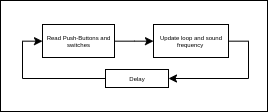
\includegraphics[scale=1.5]{Picoversatflux.pdf}}
  \vspace{0cm}\caption{Picoversat code main loop.}
  \label{fig:bd}
\end{figure}

\begin{figure}[!htbp]
  \centerline{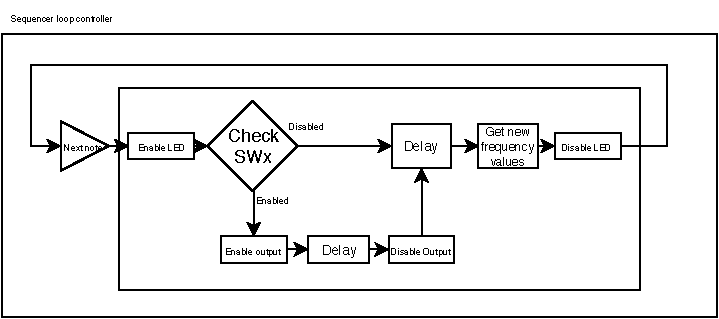
\includegraphics[scale=1]{SequencerLoopcontroler.pdf}}
  \vspace{0cm}\caption{Sequencer Loop controler peripheral main loop.}
  \label{fig:bd}
\end{figure}


\section{Block Diagram}

The hardware platform used for the developed sequencer is the Basys 2 FPGA board by digilent. The sequencer will interface with some of the board peripherals as shown in the Figure~\ref{bd} 

\begin{figure}[!htbp]
    \centerline{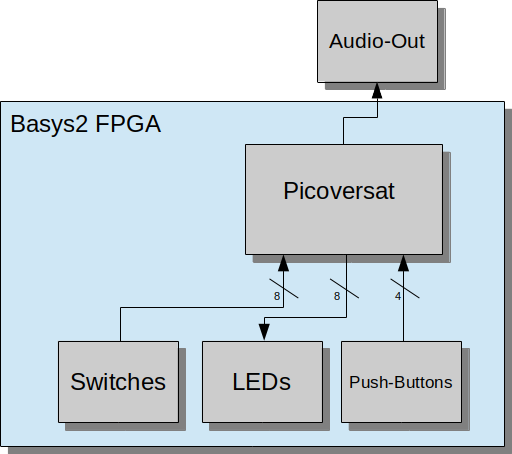
\includegraphics[scale=0.5]{bd.png}}
    \vspace{0cm}\caption{Block Diagram}
    \label{fig:bd}
\end{figure}

Figure x shows the Basys 2 peripherals that the user can use in order to interact with the sequencer

\begin{figure}[!htbp]
  \centerline{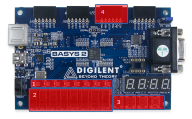
\includegraphics[scale=1]{bdboard.png}}
  \vspace{0cm}\caption{Basys 2 board peripherals}
  \label{fig:bd}
\end{figure}



attached to the data bus is shown in Figure~\ref{fig:periphs}.

\begin{figure}[!htbp]
    \centerline{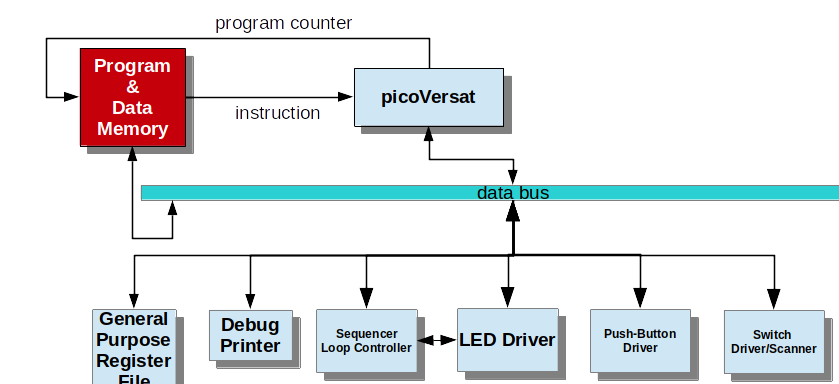
\includegraphics[width=\textwidth]{periphs.png}}
    \vspace{0cm}\caption{PicoVersat SoC with two peripherals}
    \label{fig:periphs}
\end{figure}